\section{Evaluation}
To explore the behavior of our transition matrix method under different settings, we experiment our transition matrix method with both sentence level and bag level models in the situation with and without prior knowledge of the data quality. We show that our method works in all of these settings and prior knowledge of the data quality can benefit the training of transition matrix. We also find that the sentence level models works better when we have both reliable and unreliable data, but the bag level model performs better if all the data are treated equally. Furthermore, to explore the generalization ability of our method, we also conduct experiments in two datasets.
\subsection{Data Set}
The first dataset is proposed by \cite{luo2016temporal} and aims at extraction relations between entity and time (\emph{time RE data}). The dataset is constructed by aligning Wikidata triples with Wikipedia corpus. Based on the granularity of the time expression in the sentence, this dataset can be split into 3 subsets with different levels of reliability. The reliable subset is used as basic training data, validation data and test data which contains 22,214, 2,776 and 2,771 positive sentences respectively. The two less reliable subset contains 2,094 and 53,469 positive sentences and are used as additional training data. Negative data are constructed with two heuristic strategies. We use this dataset because this is a public dataset on relation extraction that has both reliable and unreliable data, which is suitable for all of our experiment settings.

We also experiment on the dataset proposed by \cite{riedel2010modeling}, which is a commonly used dataset in relation extraction (\emph{entity RE}). This dataset is generated by aligning triples in Freebase with the New York Times corpus (NYT corpus). The training data contains 522,611 sentences and 281,270 entity pairs. The test set contains 172,448 sentences and 96,678 entity pairs. We experiment our bag level models in this dataset to see the generalization ability of our transition matrix model.

\begin{figure}[htbp]
\begin{center}
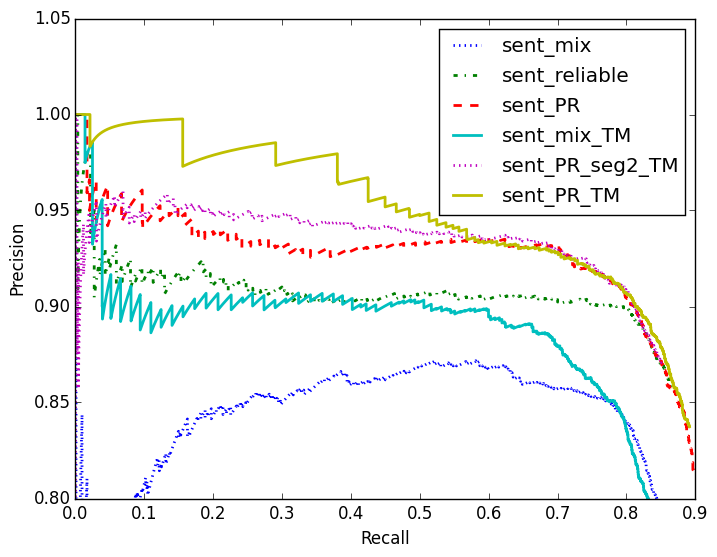
\includegraphics[width=0.9\linewidth]{figures/sent_time_exp_overall.png}
\caption{Sentence Level Results on Time RE}
\label{fig: sent_luo}
\end{center}
\end{figure}

\subsection{Hyper-parameters}
\paragraph{Sentence Level Model}
We experiment our sentence level model on time RE data. We use 100-dimensional word embedding pre-trained using GloVe \cite{pennington2014glove} on Wikipedia and Gigaword, and 20-dimensional vector for distance embedding. The convolution window is 3 and the number of convolution kernels is 200. The size of the full connection layer is also 200. As for training, we use stochastic gradient descend (SGD) with batch size 20, learning rate 0.1. We also use dropout with probability 0.5 upon the sentence embedding. Each data subset is added after 15 epochs since the precious one is added. The trace regularization parameters for three subsets are $\beta_1=-0.01$, $\beta_2=0.01$ and $\beta_3=0.1$ respectively from the reliable one to the most unreliable one (the ratio of $\beta_3$ and $\beta_2$ is fixed to 10 and 5 when tuning hyper-parameters).

\paragraph{Bag Level Model}
The parameters of the bag level model is almost the same as the sentence level model on time RE data, except that the learning rate is 0.01. As for entity RE data, The word embedding is of dimension 50 and is pre-trained on the NYT corpus using word2vec\footnote{\url{ https://code.google.com/p/word2vec/}}. The convolution window is 3 and the number of convolution kernels is 256, distance embedding size is 5, batch size is 16 and learning rate is 0.01. For all the bag level models, the linear combination parameter $\alpha$ is 1 and trace regularization parameter $\beta$ is -0.1 at the start of training. We experiment with decay rate \{0.95, 0.9, 0.8\} and decay step \{3, 5, 8\}. We find that using decay rate 0.9 and decay step 5 performs well in most situations.

\begin{figure*}[htbp]
\centering
\subfigure[Attention Aggregation]{
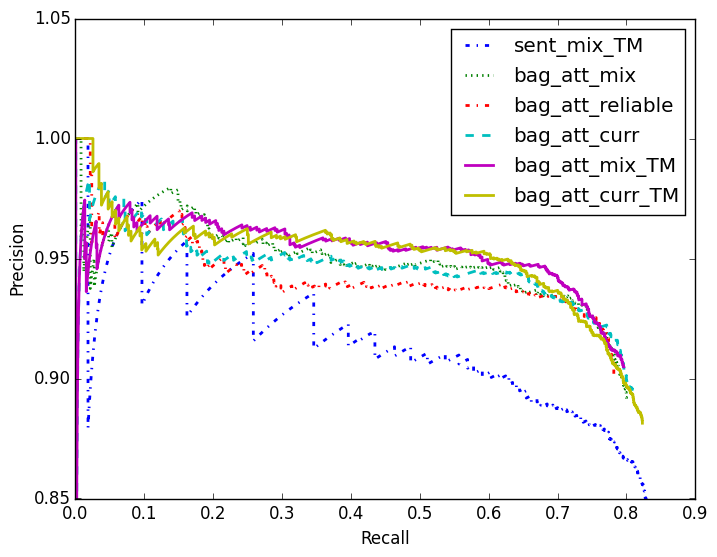
\includegraphics[width=0.45\linewidth]{figures/bag_att_exp_overall.png}
\label{fig: bag_att_luo}
}
\subfigure[Average Aggregation]{
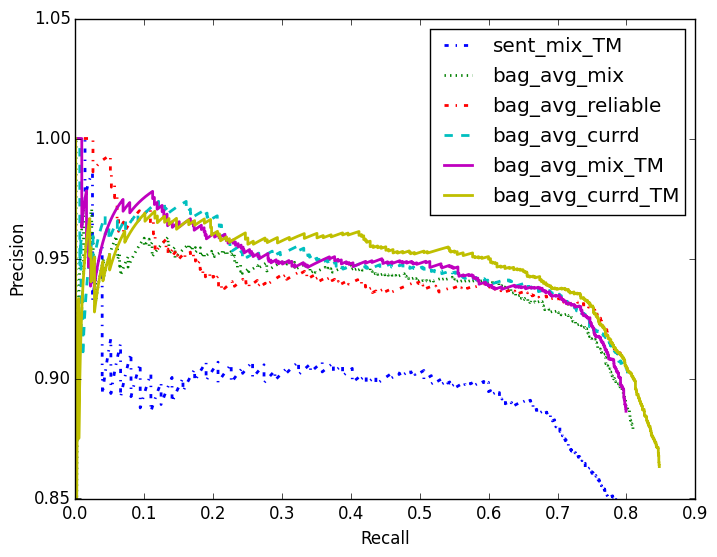
\includegraphics[width=0.45\linewidth]{figures/bag_avg_exp_overall.png}
\label{fig: bag_avg_luo}
}
\caption{Bag Level Results on Time RE}
\label{fig: results_on_luo}
\end{figure*}

\subsection{Results on Time RE Data}
\paragraph{Sentence Level Models}
The results of sentence level models are shown in Figure \ref{fig: sent_luo} in the form of precision recall curves (PR curves). We can see that the performance of the model trained on all subsets mixed together (\emph{sent\_mix}) is very bad, and is significantly worse than the model trained only on the reliable subset (\emph{sent\_reliable}), which shows that the noise problem is nonnegligible. However, with the help of transition matrix, the model obtains the ability of modeling noise (\emph{sent\_mix\_TM}), which significantly improves the performance of the model. By using the reliable subset first and gradually adding less reliable data (\emph{sent\_currd\footnote{\emph{curr} refers to curriculum learning and \emph{d} refers to data}}), we can see that the model can actually make use of the noisy data and performs better than the model trained only on the reliable subset. However, by mixing the two unreliable subsets together and use the curriculum of training on the reliable data first as well as the transition matrix, we can see that the prior knowledge of data quality can help the transition matrix model the noise better and further improve the model performance. Furthermore, by using the curriculum of 3 subsets (\emph{sent\_currd\_TM}) instead of 2, the performance can be further improved. Therefore, we will use 3 subsets in the rest of the experiments.

\paragraph{Bag Level Attention Aggregation Models}
The results of the bag level models with attention aggregation is shown in Figure \ref{fig: bag_att_luo}. We can see that the basic bag level attention aggregation model (\emph{bag\_att\_mix}) performs good and significantly outperforms the \emph{sent\_mix\_TM} model. Recall that the bag level model is based on the \emph{at-least-one assumption} that at least one of the sentences in the sentence bag support the ($subj$, $rel$, $obj$) triple, and the \emph{sent\_mix\_TM} model do not use any assumption about the dataset. This shows that prior knowledge of the data quality plays an important role in the situation where the dataset is noisy. We can see that the model trained only on the reliable subset (\emph{bag\_att\_reliable}) performs worse than the model trained on the mixed dataset, which shows that the attention aggregation has some denoising ability and can make use of the noisy data. However, since attention aggregation already has reasonable denoising ability, we can see that although adding noisy data gradually alone works well in sentence level model, it does not improve the attention aggregation model (\emph{bag\_att\_currd}). Note that the at-least-one assumption does not always hold and there are also false negative and false positive problems in bag level. Therefore, we can see that using transition matrix with or without curriculum learning over the dataset (\emph{bag\_att\_currd\_TM} and \emph{bag\_att\_mix\_TM}) all improve the model performance, and \emph{bag\_att\_currd\_TM} performs slightly better.

\paragraph{Bag Level Average Aggregation Models}
The results of the bag level models with average aggregation is shown in Figure \ref{fig: bag_avg_luo}. The ranking of each setting is similar to the attention aggregation models. However, since its denoising ability is not as good as attention aggregation, adding unreliable data gradually (\emph{bag\_avg\_currd}) improves the model performance here. We can also see that the transition matrix improves the average aggregation models more significantly than the attention aggregation models. Note that due to the inferior denoising ability of average aggregation, the unhandled sentence level noise may further propagates to bag level, which gives the transition matrix more chance to help model the noise.
 
\begin{figure}[htbp]
\begin{center}
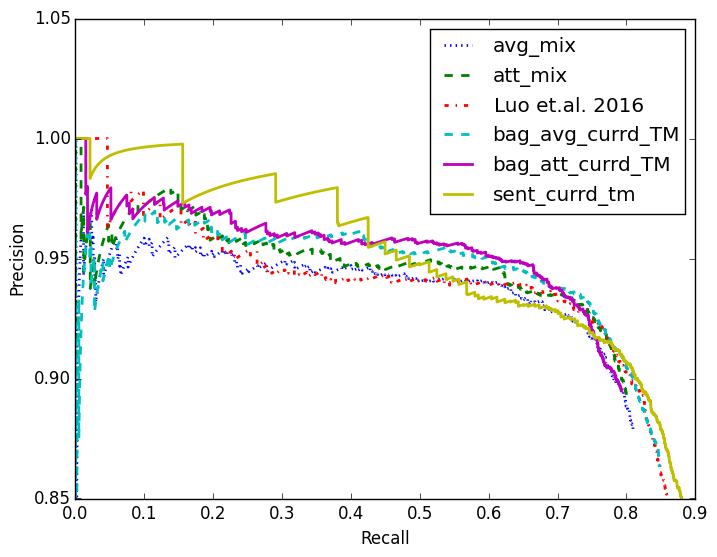
\includegraphics[width=0.9\linewidth]{figures/best_cmp_exp_overall.png}
\caption{Comparison on Time RE}
\label{fig: cmp_luo}
\end{center}
\end{figure}
 
\paragraph{Comparison}
The comparison of the best settings of each model family is shown in Figure \ref{fig: cmp_luo}. We can see that all of our transition matrix models outperform the model of \cite{luo2016temporal}. With the help of transition matrix, although the basic version of average aggregation is not as good as attention aggregation, its transition matrix version is similar to the attention aggregation. Also note that although the sentence level models trained on mixed data do not perform very good, the sentence level model can use transition matrix to model the sentence level noise and thus performs best in all these models. Recall that the transition matrix can model the noise rather than just reduce the influence of noisy sentences as in bag level models, the sentence level model actually has the ability to make use of the noisy data. This shows that sentence level noise is more significant than the bag level noise in relation extraction, and modeling noise works better than just trying to reducing the influence of noise.


\begin{figure}[htbp]
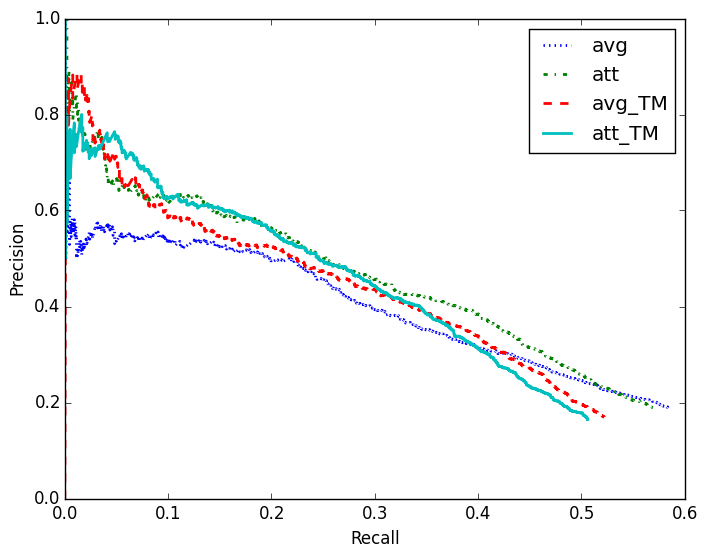
\includegraphics[width=0.9\linewidth]{figures/re_att_avg_cmp_exp.png}
\caption{Results on Dataset of Riedel et.al.} 
\label{fig: Riedel_res}
\end{figure}

\subsection{Performance on Entity RE Data}
To show the generalization ability of our proposed transition matrix method, we also conduct experiments on the entity RE dataset proposed by \cite{riedel2010modeling}. We implement the average aggregation method (\emph{avg}) and the attention aggregation method (\emph{att}) proposed by \cite{lin2016neural} as well as their corresponding transition matrix versions (\emph{avg\_TM} and \emph{att\_TM}). The results are shown in Figure \ref{fig: Riedel_res}. We can see that, due to the inferior denoising ability of average aggregation, it performs significantly worse than attention aggregation. Similar to the results in time RE data, since the unhandled sentence level noise propagates to the bag level, which makes the bag level noise become more severe, the transition matrix has more chance to model the noise. Therefore, the \emph{avg\_TM} model clearly outperforms the \emph{avg} model. As for attention aggregation, this model already have good ability in reducing the impact of sentence level noise. Since the bag level noise is less significant than the sentence level noise, the improvement of our transition matrix model is limited, which only improves the model on the low recall part. Note that the low recall part corresponds to high precision, which is more useful than the rest of the extraction results in practice. Therefore, our transition matrix method is also useful in this situation.

\iffalse
\begin{figure*}[htbp]
\centering
\subfigure[Overall PR Curves]{
\includegraphics[width=0.475\linewidth]{reg_exp_overall.png}
\label{fig: reg_overall_pr_curve}
}
\subfigure[Small Relation PR Curves]{
\includegraphics[width=0.475\linewidth]{reg_exp_small.png}
\label{fig: reg_small_rel_pr_curve}
}
\caption{Imapct of Regularization Weights} 
\label{fig: reg_PR_curve}
\end{figure*}
\fi
